
\chapter{Kravspecifikation}
\section{Godkendelsesformular}
\begin{table}[h!]
\label{tab:tabel2}
\begin{tabular}{| l | >{\raggedright\arraybackslash}p{12cm} |}
   \hline
   \textbf{Forfattere} & Line, Mette, Brian, Mohamed, Khaled og Ida\\ \hline
   \textbf{Godkendes af:} & Samuel Alberg Thrysøe\\ \hline
   \textbf{Antal sider:} & \\ \hline
   \textbf{Kunde:} & IHA\\ \hline
\end{tabular}
\end{table}
\textbf{Ved underskrivelse af dette dokument accepteres det af begge parter, som værende kravene til udviklingen af det ønskede system.}
\newline
\textbf{Sted og dato:}\\
\\
\\
\begin{table}
[h!]
\begin{tabular}{ l lllllllll l}
--------------------------------------&&&&&&&&&&--------------------------------------\\ 
Kundens underskrift &&&&&&&&&&Leverandørens underskrift\\
\end{tabular}
\end{table}
\section{Indledning}

\section{Systembeskrivelse}

\section{Aktør-kontekst diagram}
\begin{figure}[h!]
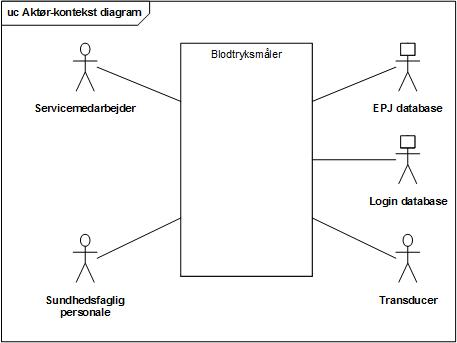
\includegraphics[width =1.0\textwidth , right]{billeder/Aktorkontekst.jpg}
\end{figure}
\section{Use cases}
\begin{figure}[h!]
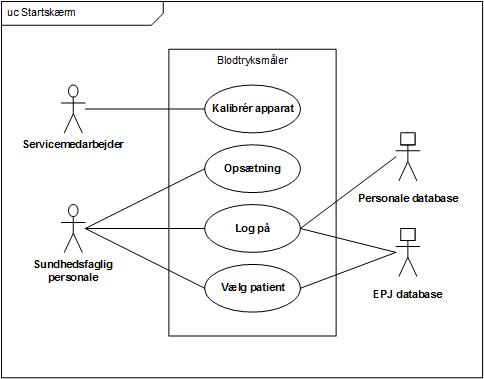
\includegraphics[width =1.0\textwidth , right]{billeder/UCStart}
\end{figure}
\begin{figure}[h!]
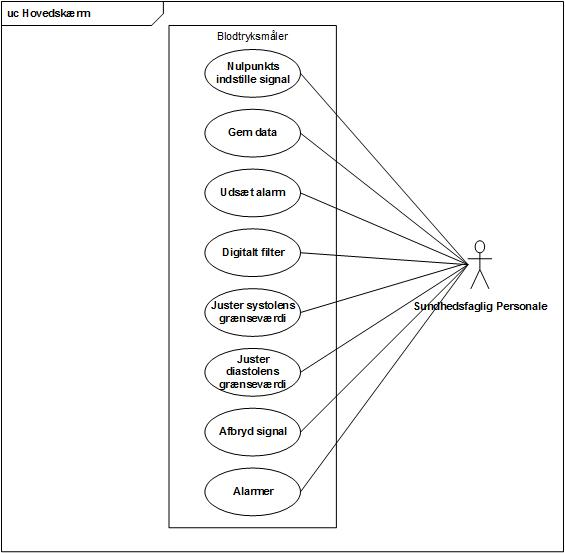
\includegraphics[width =1.0\textwidth , right]{billeder/UChoved}
\end{figure}
\begin{table}[h!]
\caption{Use case 1}\label{tab:tabel3}
\begin{tabular}{| l | >{\raggedright\arraybackslash}p{11cm} |}
   \hline
   \textbf{Use case 1} & \textbf{Kalibrer apparat}\\ \hline
   Mål: & Få kalibreret apparatet \\ \hline
   Initiering: & Startes af Servicemedarbejder\\ \hline
   Aktører:& Servicemedarbejder (primær)\\ \hline
   Referencer: & - \\ \hline
   Samtidige forekomster: & én kalibrering pr. apparat \\\hline
   Forudsætninger: & Blodtryksmålersystemet er tændt og tilsluttet kalibreringsudstyret.\\ \hline
   Resultat:& Apparatet er kalibreret\\ \hline
   Hovedscenarie:& 
1. Tryk på "Kalibrering"\newline
2. Systemet starter kalibreringen\newline
3. Besked: "Kalibreringen er fuldendt" vises på GUI\\\hline
Udvidelse/undtagelser: & - \\\hline
\end{tabular}
\end{table}


\begin{table}[h!]
\caption{Use case 2}\label{tab:tabel3}
\begin{tabular}{| l | >{\raggedright\arraybackslash}p{11cm} |}
   \hline
   \textbf{Use case 2} & \textbf{Start måling}\\ \hline
   Mål: & Få indsendt signalerne fra patienten, startet analysen samt skiftet til hovedskærmen \\ \hline
   Initiering: & Startes af Sundhedsfaglig personale\\ \hline
   Aktører:& Sundhedsfaglig personale (primær), Transducer (sekundær)\\ \hline
   Referencer: & Use case 1 og Use case 11 \\ \hline
   Samtidige forekomster: & Én transducer pr. måling \\\hline
   Forudsætninger: & Blodtryksmålersystemet er tændt. Use case 11 er kørt succesfuldt. Sundhedsfaglig personale ID. er indtastet. \\ \hline
   Resultat:& Tranducerens data vises i GUI\\ \hline
   Hovedscenarie:& 
1. Tryk på "Start" på startskærm \newline
2. Kommer ind på hovedskærmen \newline
   $[$Undtagelse 1: Ingen data indhentet$]$\newline
3. Systemet indhenter data \newline
3. EKG, blodtrykskurve og iltmætningskurve præsenteres kontinuert på en graf. Puls, Systolisk, diastolisk, middeltryk og iltmætning vises som talværdier på GUI. \\\hline
Udvidelse/undtagelser: & $[$ Undtagelse 1: Ingen data indhentet$]$\newline
1.1 Intet data er indhentet\newline
1.2 Use case afsluttes\\\hline
\end{tabular}
\end{table}


\begin{table}[h!]
\caption{Use case 3}\label{tab:tabel3}
\begin{tabular}{| l | >{\raggedright\arraybackslash}p{11cm} |}
   \hline
   \textbf{Use case 3} & \textbf{Nulpunkts indstille signal}\\ \hline
   Mål: & Få nulpunkts indstillet signalerne, sådan at signalerne ligger korrekte på deres akse. \\ \hline
   Initiering: & Startes af Sundhedsfaglig personale\\ \hline
   Aktører:& Sundhedsfaglig personale (primær)\\ \hline
   Referencer: & Use case 2\\ \hline
   Samtidige forekomster: & -  \\\hline
   Forudsætninger: & Use case 2 er kørt succesfuldt\\ \hline
   Resultat:& Signalet er nulpunkts indstillet\\ \hline
   Hovedscenarie:& 
1. Tryk på "Nulpunks indstilling"\newline
2. Systemet starter nulpunkts indstillingen\newline
3. Besked "Nulpunkts indstillingen er fuldent" vises på GUI\\\hline
Udvidelse/undtagelser: & - \\\hline
\end{tabular}
\end{table}

\begin{table}[h!]
\caption{Use case 4}\label{tab:tabel3}
\begin{tabular}{| l | >{\raggedright\arraybackslash}p{11cm} |}
   \hline
   \textbf{Use case 4} & \textbf{Gem data}\\ \hline
   Mål: &  Få gemt EKG, blodtrykskurve, iltmætningskurve, puls, systole, diastole, middeltryk og iltmætning i databasen \\ \hline
   Initiering: & Startes af Sundhedsfaglig personale\\ \hline
   Aktører:& Sundhedsfaglig personale (primær), Database (sekundær)\\ \hline
   Referencer: & Use Case 2\\ \hline
   Samtidige forekomster: & - \\\hline
   Forudsætninger: & Use case 2 er kørt succesfuldt  \\ \hline
   Resultat:& Patientens data er gemt i database\\ \hline
   Hovedscenarie:& 
1. Tryk på "Gem"\newline
   $[$Undtagelse 1: Intet CPR koblet til data$]$\newline
2. Systemet gemmer EKG, blodtrykskurve, iltmætningskurve, puls, systole, diastole, middeltryk og iltmætning i database\newline
3. Besked "Data med CPR gemt" vises på GUI \\\hline
Udvidelse/undtagelser: & $[$Undtagelse 1: Intet CPR koblet til data$]$\newline
1.1. Indtast patientens CPR i pop-up vindue\newline
1.2. Tryk på "Næste"\newline
1.3. Systemet gemmer EKG, blodtrykskurve, iltmætningskurve, puls, systole, diastole, middeltryk og iltmætning i database.\newline
1.4. Use case afsluttet \\\hline
\end{tabular}
\end{table}

\begin{table}[h!]
\caption{Use case 5}\label{tab:tabel3}
\begin{tabular}{| l | >{\raggedright\arraybackslash}p{11cm} |}
   \hline
   \textbf{Use case 5} & \textbf{Udsæt alarm}\\ \hline
   Mål: & Få udsat alarmens lyd i et minut \\ \hline
   Initiering: & Startes af Sundhedsfaglig personale\\ \hline
   Aktører:& Sundhedsfaglig personale (primær) \\ \hline
   Referencer: & Use case 10 \\ \hline
   Samtidige forekomster: & \\\hline
   Forudsætninger: & Use case 10: Alarmer, er igangsat \\ \hline
   Resultat:& Alarmens lyd er stoppet et minut\\ \hline
   Hovedscenarie:& 
1. Tryk på "Udsæt alarm"\newline
2. Systemet stopper alarmens lyd i et minut \\\hline
Udvidelse/undtagelser: & -\\\hline
\end{tabular}
\end{table}

\begin{table}[h!]
\caption{Use case 6}\label{tab:tabel3}
\begin{tabular}{| l | >{\raggedright\arraybackslash}p{11cm} |}
   \hline
   \textbf{Use case 6} & \textbf{Digitalt filter}\\ \hline
   Mål: &  Få slået det digitale filter til eller fra \\ \hline
   Initiering: & Startes af Sundhedsfaglig personale\\ \hline
   Aktører:& Sundhedsfaglig personale (primær)\\ \hline
   Referencer: & Use case 2 \\ \hline
   Samtidige forekomster: & - \\\hline
   Forudsætninger: & Use case 2 er kørt succesfuldt\\ \hline
   Resultat:& Det digitale filter er slået til eller fra\\ \hline
   Hovedscenarie:& 
1. Tryk på "Digitalt filter OFF" \newline
2. Systemet slår det digitale filter fra\newline
3. Tryk på "Digitalt filter ON"\newline
4. Systemet slår det digitale filter til\\\hline
Udvidelse/undtagelser: & -\\\hline
\end{tabular}
\end{table}

\begin{table}[h!]
\caption{Use case 7}\label{tab:tabel3}
\begin{tabular}{| l | >{\raggedright\arraybackslash}p{11cm} |}
   \hline
   \textbf{Use case 7} & \textbf{Juster systolens grænseværdi}\\ \hline
   Mål: & Få flyttet grænseværdi intervallet for systolen op eller ned \\ \hline
   Initiering: & Startes af Sundhedsfaglig personale\\ \hline
   Aktører:& Sundhedsfaglig personale (primær)\\ \hline
   Referencer: & Use case 2 \\ \hline
   Samtidige forekomster: & \\\hline
   Forudsætninger: & Use case 2 er kørt succesfuldt\\ \hline
   Resultat:& Grænseværdi intervallet for systolen er justeret og intervals værdierne vises i GUI. \\ \hline
   Hovedscenarie:& 
1. Tryk på "Systole op"\newline
2. Grænseværdien ændres 2.5mmHg op og intervallet vises i GUI\newline
3. Tryk på "Systole ned"\newline
4. Grænseværdien ændres 2.5mmHg ned og intervallet vises i GUI\\\hline
Udvidelse/undtagelser: & -\\\hline
\end{tabular}
\end{table}

\begin{table}[h!]
\caption{Use case 8}\label{tab:tabel3}
\begin{tabular}{| l | >{\raggedright\arraybackslash}p{11cm} |}
   \hline
   \textbf{Use case 8} & \textbf{Juster diastolens grænseværdi}\\ \hline
   Mål: &  Få flyttet grænseværdi intervallet for diastolen op eller ned\\ \hline
   Initiering: & Startes af Sundhedsfaglig personale \\ \hline
   Aktører: & Sundhedsfaglig personale (primær) \\ \hline
   Referencer: & Use case 2\\ \hline
   Samtidige forekomster: & - \\\hline
   Forudsætninger: & Use case 2 er kørt succesfuldt\\ \hline
   Resultat:& Grænseværdi intervallet for diastolen er justeret og intervals værdierne vises i GUI.\\ \hline
   Hovedscenarie:& 
1. Tryk "Diastole op"\newline
2. Diastolens grænseværdi ændres 2.5mmHg op og intervellet vises i GUI\newline
3. Tryk "Diastole ned"\newline
4. Diastolens grænseværdi ændres 2.5mmHg ned og intervellet vises i GUI\\\hline
Udvidelse/undtagelser: & -\\\hline
\end{tabular}
\end{table}

\begin{table}[h!]
\caption{Use case 9}\label{tab:tabel3}
\begin{tabular}{| l | >{\raggedright\arraybackslash}p{11cm} |}
   \hline
   \textbf{Use case 9} & \textbf{Afbryd signal}\\ \hline
   Mål: & Få afbrudt signalet og vendt tilbage til startskærmen. \\ \hline
   Initiering: & Startes af Sundhedsfaglig personale\\ \hline
   Aktører:& Sundhedsfaglig personale (primær) \\ \hline
   Referencer: & Use case 2\\ \hline
   Samtidige forekomster: & - \\\hline
   Forudsætninger: & Use case 2 er kørt succesfuldt \\ \hline
   Resultat:& Afbrudt signalet og vendt tilbage til startskærmen \\ \hline
   Hovedscenarie:& 
1. Tryk på "AFBRYD" \newline
2. Pop-up vindue kommer op: "Er du sikker"\newline
3. Tryk på "Ja"\newline
   $[$Udvidelse 1: Tryk på "Nej"$]$\newline
5. Startkærmen kommer frem og ny måling kan foretages\\\hline
Udvidelse/undtagelser: & $[$Udvidelse 1: Tryk på "Nej"$]$\newline
1.1 Tryk "Nej"\newline
1.2 Kommer tilbage til hovedskærmen\newline
1.3 Use case afsluttet\\\hline
\end{tabular}
\end{table}


\begin{table}[h!]
\caption{Use case 10}\label{tab:tabel3}
\begin{tabular}{| l | >{\raggedright\arraybackslash}p{11cm} |}
   \hline
   \textbf{Use case 10} & \textbf{Alarmer}\\ \hline
   Mål: & Få startet alarmeringen ved overskridelse af grænseværdi \\ \hline
   Initiering: & Systemet starter denne Use case\\ \hline
   Aktører:& Sundhedsfaglig personale (sekundær)\\ \hline
   Referencer: & Use case 2 \\ \hline
   Samtidige forekomster: & - \\\hline
   Forudsætninger: & Målingen i Use case 2 er kørt succesfuldt \\ \hline
   Resultat:& Alarmen starter\\ \hline
   Hovedscenarie:& 
1. Grænseværdi overskrides \newline
2. Grænseværdi er overskredet\newline
3. Alarm starter med lyd og tallet som har overskredet grænseværdien blinker.\newline
    $[$Udvidelse 1: Anden grænseværdi overskrides$]$ 
\\\hline
Udvidelse/undtagelser: & $[$Udvidelse 1: Anden grænseværdi overskrides$]$ \newline
1.1. Endnu en grænseværdi overskrides\newline
1.2. Lyden fra første alarm fortsætter. Det nye tal som har overskredet grænseværdien blinker ligeledes.\newline
1.3 Use case afsluttet.\\\hline
\end{tabular}
\end{table}


\begin{table}[h!]
\caption{Use case 11}\label{tab:tabel3}
\begin{tabular}{| l | >{\raggedright\arraybackslash}p{11cm} |}
   \hline
   \textbf{Use case 15} & \textbf{Opsætning}\\ \hline
   Mål: & Få valgt port til NI-DAQ \\ \hline
   Initiering: & startes af Sundhedsfaglig personalee\\ \hline
   Aktører:& Sundhedsfaglig personale (primær) \\ \hline
   Referencer: &  -\\ \hline
   Samtidige forekomster: & Ét blodtryksmålersystem pr. opsætning \\\hline
   Forudsætninger: & Tilsluttet en computer. \\ \hline
   Resultat:& Port valgt\\ \hline
   Hovedscenarie:& 
1. Tryk på dropdown på startskærmen\newline
2. Port vælges \\\hline
Udvidelse/undtagelser: & -\\\hline
\end{tabular}
\end{table}



\section{Ikke-funktionelle krav}

\chapter{Accepttest}
\section{Indledning}
\section{Accepttest for funktionelle krav}

\subsection{Opstilling}
Billede indsættes - haves ikke endnu

\begin{table}[h!]
\caption{Accepttest for Use case 1}\label{tab:tabel8}
\begin{tabular}{|>{\raggedright\arraybackslash}p{2.5cm}| >{\raggedright\arraybackslash}p{2.9cm} | >{\raggedright\arraybackslash}p{2.9cm} | >{\raggedright\arraybackslash}p{2.9cm} | >{\raggedright\arraybackslash}p{2.8cm} |}
   \hline
   \textbf{Use case 1: Kalibrer apparatur} &\textbf{Test}& \textbf{Forventet resultat} & \textbf{Visuelt resultat} & \textbf{Godkendt/ kommentar}\\ \hline
   Normalforløb:& Tryk på "Kalibrering" &Systemet er kalibreret & besked "Kalibreringen er fuldendt" &\\\hline
\end{tabular}
\end{table}



\begin{table}[h!]
\caption{Accepttest for Use case 2}\label{tab:tabel8}
\begin{tabular}{|>{\raggedright\arraybackslash}p{2.5cm}| >{\raggedright\arraybackslash}p{2.9cm} | >{\raggedright\arraybackslash}p{2.9cm} | >{\raggedright\arraybackslash}p{2.9cm} | >{\raggedright\arraybackslash}p{2.8cm} |}
   \hline
   \textbf{Use case 2: Start måling } &\textbf{Test}& \textbf{Forventet resultat} & \textbf{Visuelt resultat} & \textbf{Godkendt/ kommentar}\\ \hline
   Normalforløb:& Tryk på "Start" & EKG, Blodtrykskurve og iltmætningskurver vises kontinuert på en graf. \newline Puls, systolisk, diastolisk, middeltryk og iltmætnings vises som talværdier på GUI & Tal og grafer vises på GUI &\\\hline
\end{tabular}
\end{table}

\begin{table}[h!]
\caption{Accepttest for Use case 3}\label{tab:tabel8}
\begin{tabular}{|>{\raggedright\arraybackslash}p{2.5cm}| >{\raggedright\arraybackslash}p{2.9cm} | >{\raggedright\arraybackslash}p{2.9cm} | >{\raggedright\arraybackslash}p{2.9cm} | >{\raggedright\arraybackslash}p{2.8cm} |}
   \hline
   \textbf{Use case 3: Nulpunkts indstille signal } &\textbf{Test}& \textbf{Forventet resultat} & \textbf{Visuelt resultat} & \textbf{Godkendt/ kommentar}\\ \hline
   Normalforløb:& Tryk på "Nulpunkts indstilling" & Blodtrykskurven nulpunkts indstilles & Besked " Nulpunkts indstilling er fuldendt" &\\\hline
\end{tabular}
\end{table}

\begin{table}[h!]
\caption{Accepttest for Use case 4}\label{tab:tabel8}
\begin{tabular}{|>{\raggedright\arraybackslash}p{2.5cm}| >{\raggedright\arraybackslash}p{2.9cm} | >{\raggedright\arraybackslash}p{2.9cm} | >{\raggedright\arraybackslash}p{2.9cm} | >{\raggedright\arraybackslash}p{2.8cm} |}
   \hline
   \textbf{Use case 4: Gem data } &\textbf{Test}& \textbf{Forventet resultat} & \textbf{Visuelt resultat} & \textbf{Godkendt/ kommentar}\\ \hline
   Normalforløb:& Tryk på "Gem" & Data gemmes i database & Besked "Data med CPR gemt"&\\\hline
\end{tabular}
\end{table}


\begin{table}[h!]
\caption{Accepttest for Use case 5}\label{tab:tabel8}
\begin{tabular}{|>{\raggedright\arraybackslash}p{2.5cm}| >{\raggedright\arraybackslash}p{2.9cm} | >{\raggedright\arraybackslash}p{2.9cm} | >{\raggedright\arraybackslash}p{2.9cm} | >{\raggedright\arraybackslash}p{2.8cm} |}
   \hline
   \textbf{Use case 5: Udsæt alarm } &\textbf{Test}& \textbf{Forventet resultat} & \textbf{Visuelt resultat} & \textbf{Godkendt/ kommentar}\\ \hline
   Normalforløb:& Tryk "Udsæt alarm" & Alarmens lyd stopper & Den overskredede værdi blinker &\\\hline
\end{tabular}
\end{table}



\begin{table}[h!]
\caption{Accepttest for Use case 6}\label{tab:tabel8}
\begin{tabular}{|>{\raggedright\arraybackslash}p{2.5cm}| >{\raggedright\arraybackslash}p{2.9cm} | >{\raggedright\arraybackslash}p{2.9cm} | >{\raggedright\arraybackslash}p{2.9cm} | >{\raggedright\arraybackslash}p{2.8cm} |}
   \hline
   \textbf{Use case 6: Digitalt filter } &\textbf{Test}& \textbf{Forventet resultat} & \textbf{Visuelt resultat} & \textbf{Godkendt/ kommentar}\\ \hline
   Normalforløb:& Tryk på "Digitalt filter OFF" & Det digitale filter er slået fra & Data er ufiltreret og knappen ændrer navn &\\\hline
   &Tryk på "Digitalt filter ON" &Det digitale filter er slået til &Data er filtreret og knappen ændrer navn. &\\\hline
\end{tabular}
\end{table}


\begin{table}[h!]
\caption{Accepttest for Use case 7}\label{tab:tabel8}
\begin{tabular}{|>{\raggedright\arraybackslash}p{2.5cm}| >{\raggedright\arraybackslash}p{2.9cm} | >{\raggedright\arraybackslash}p{2.9cm} | >{\raggedright\arraybackslash}p{2.9cm} | >{\raggedright\arraybackslash}p{2.8cm} |}
   \hline
   \textbf{Use case 7: Juster systolens grænseværdi } &\textbf{Test}& \textbf{Forventet resultat} & \textbf{Visuelt resultat} & \textbf{Godkendt/ kommentar}\\ \hline
   Normalforløb:& Tryk på "Systole op"& Grænseværdien ændres 2.5mmHg op & Talværdierne ændrer sig på GUI &\\\hline
   &Tryk på "Systole ned" & Grænseværdien ændres 2.5 mmHg ned & Talværdierne ændrer sig på GUI & \\\hline
\end{tabular}
\end{table}


\begin{table}[h!]
\caption{Accepttest for Use case 8}\label{tab:tabel8}
\begin{tabular}{|>{\raggedright\arraybackslash}p{2.5cm}| >{\raggedright\arraybackslash}p{2.9cm} | >{\raggedright\arraybackslash}p{2.9cm} | >{\raggedright\arraybackslash}p{2.9cm} | >{\raggedright\arraybackslash}p{2.8cm} |}
   \hline
   \textbf{Use case 8: Juster diastolens grænseværdi } &\textbf{Test}& \textbf{Forventet resultat} & \textbf{Visuelt resultat} & \textbf{Godkendt/ kommentar}\\ \hline
   Normalforløb:&Tryk på "Diastole op"  & Grænseværdien ændres 2.5mmHg op & Talværdierne ændrer sig på GUI &\\\hline
   &Tryk på "Diastole ned" & Grænseværdien ændres 2.5 mmHg ned & Talværdierne ændrer sig på GUI &\\\hline
\end{tabular}
\end{table}

\begin{table}[h!]
\caption{Accepttest for Use case 9}\label{tab:tabel8}
\begin{tabular}{|>{\raggedright\arraybackslash}p{2.5cm}| >{\raggedright\arraybackslash}p{2.9cm} | >{\raggedright\arraybackslash}p{2.9cm} | >{\raggedright\arraybackslash}p{2.9cm} | >{\raggedright\arraybackslash}p{2.8cm} |}
   \hline
   \textbf{Use case 9: Afbryd signalet } &\textbf{Test}& \textbf{Forventet resultat} & \textbf{Visuelt resultat} & \textbf{Godkendt/ kommentar}\\ \hline
   Normalforløb:& Tryk "AFBRYD" & Pop-up vindue dukker op & Pop-up skærm: "Er du sikker?" &\\\hline
   &Tryk "Ja"&Tilbage til startskærmen& Startskærmen kommer frem&\\\hline
\end{tabular}
\end{table}

\begin{table}[h!]
\caption{Accepttest for Use case 10}\label{tab:tabel8}
\begin{tabular}{|>{\raggedright\arraybackslash}p{2.5cm}| >{\raggedright\arraybackslash}p{2.9cm} | >{\raggedright\arraybackslash}p{2.9cm} | >{\raggedright\arraybackslash}p{2.9cm} | >{\raggedright\arraybackslash}p{2.8cm} |}
   \hline
   \textbf{Use case 10: Alarmer } &\textbf{Test}& \textbf{Forventet resultat} & \textbf{Visuelt resultat} & \textbf{Godkendt/ kommentar}\\ \hline
   Normalforløb:& Grænseværdi overskrides& Alarmen starter med lyd og talværdien som har overskredet grænseværdien blinker & Tal blinker &\\\hline
\end{tabular}
\end{table}

\begin{table}[h!]
\caption{Accepttest for Use case 11}\label{tab:tabel8}
\begin{tabular}{|>{\raggedright\arraybackslash}p{2.5cm}| >{\raggedright\arraybackslash}p{2.9cm} | >{\raggedright\arraybackslash}p{2.9cm} | >{\raggedright\arraybackslash}p{2.9cm} | >{\raggedright\arraybackslash}p{2.8cm} |}
   \hline
   \textbf{Use case 11: Opsætning } &\textbf{Test}& \textbf{Forventet resultat} & \textbf{Visuelt resultat} & \textbf{Godkendt/ kommentar}\\ \hline
   Normalforløb:& Tryk på dropdown og vælg port & Port vælges & Port valgt &\\\hline
\end{tabular}
\end{table}


\newpage

\newpage

\newpage

\newpage

\section{Accepttest for ikke-funktionelle krav}

\begin{longtable}{|>{\raggedright\arraybackslash}p{1.1cm}| >{\raggedright\arraybackslash}p{2.7cm} | >{\raggedright\arraybackslash}p{2.7cm} | >{\raggedright\arraybackslash}p{2.7cm} | >{\raggedright\arraybackslash}p{2.2cm} |>{\raggedright\arraybackslash}p{2.2cm}|}
   \caption{Accepttest for ikke-funktionelle krav}\label{tab:label13}
\\ \hline   
\textbf{Krav nr.}&\textbf{Krav} &\textbf{Test}& \textbf{Forventet resultat} & \textbf{Resultat} & \textbf{Godkendt/ kommentar}\\ \hline
   & & & & & \\\hline
   & & & & & \\\hline
   & & & & & \\\hline
   & & & & & \\\hline
   & & & & & \\\hline
   & & & & & \\\hline
\end{longtable}

\section{Godkendelses formular}
\begin{table}[h!]
\label{tab:tabel14}
\begin{tabular}{| l | >{\raggedright\arraybackslash}p{12cm} |}
   \hline
   \textbf{Dato for test} &\\ \hline
   \textbf{Godkendes af:} & \\ \hline
\end{tabular}
\end{table}
\textbf{Ved underskrivelse af dette dokument godkendes den kørte accepttest}
\newline
\textbf{Sted og dato:}\\
\\
\\
\begin{table}
[h!]
\begin{tabular}{ l lllllllll l}
--------------------------------------&&&&&&&&&&--------------------------------------\\ 
Kundens underskrift &&&&&&&&&&Leverandørens underskrift\\
\end{tabular}
\end{table}